% Options for packages loaded elsewhere
\PassOptionsToPackage{unicode}{hyperref}
\PassOptionsToPackage{hyphens}{url}
%
\documentclass[
  ignorenonframetext,
]{beamer}
\usepackage{pgfpages}
\setbeamertemplate{caption}[numbered]
\setbeamertemplate{caption label separator}{: }
\setbeamercolor{caption name}{fg=normal text.fg}
\beamertemplatenavigationsymbolsempty
% Prevent slide breaks in the middle of a paragraph
\widowpenalties 1 10000
\raggedbottom
\setbeamertemplate{part page}{
  \centering
  \begin{beamercolorbox}[sep=16pt,center]{part title}
    \usebeamerfont{part title}\insertpart\par
  \end{beamercolorbox}
}
\setbeamertemplate{section page}{
  \centering
  \begin{beamercolorbox}[sep=12pt,center]{part title}
    \usebeamerfont{section title}\insertsection\par
  \end{beamercolorbox}
}
\setbeamertemplate{subsection page}{
  \centering
  \begin{beamercolorbox}[sep=8pt,center]{part title}
    \usebeamerfont{subsection title}\insertsubsection\par
  \end{beamercolorbox}
}
\AtBeginPart{
  \frame{\partpage}
}
\AtBeginSection{
  \ifbibliography
  \else
    \frame{\sectionpage}
  \fi
}
\AtBeginSubsection{
  \frame{\subsectionpage}
}
\usepackage{amsmath,amssymb}
\usepackage{lmodern}
\usepackage{iftex}
\ifPDFTeX
  \usepackage[T1]{fontenc}
  \usepackage[utf8]{inputenc}
  \usepackage{textcomp} % provide euro and other symbols
\else % if luatex or xetex
  \usepackage{unicode-math}
  \defaultfontfeatures{Scale=MatchLowercase}
  \defaultfontfeatures[\rmfamily]{Ligatures=TeX,Scale=1}
\fi
% Use upquote if available, for straight quotes in verbatim environments
\IfFileExists{upquote.sty}{\usepackage{upquote}}{}
\IfFileExists{microtype.sty}{% use microtype if available
  \usepackage[]{microtype}
  \UseMicrotypeSet[protrusion]{basicmath} % disable protrusion for tt fonts
}{}
\makeatletter
\@ifundefined{KOMAClassName}{% if non-KOMA class
  \IfFileExists{parskip.sty}{%
    \usepackage{parskip}
  }{% else
    \setlength{\parindent}{0pt}
    \setlength{\parskip}{6pt plus 2pt minus 1pt}}
}{% if KOMA class
  \KOMAoptions{parskip=half}}
\makeatother
\usepackage{xcolor}
\newif\ifbibliography
\usepackage{color}
\usepackage{fancyvrb}
\newcommand{\VerbBar}{|}
\newcommand{\VERB}{\Verb[commandchars=\\\{\}]}
\DefineVerbatimEnvironment{Highlighting}{Verbatim}{commandchars=\\\{\}}
% Add ',fontsize=\small' for more characters per line
\usepackage{framed}
\definecolor{shadecolor}{RGB}{248,248,248}
\newenvironment{Shaded}{\begin{snugshade}}{\end{snugshade}}
\newcommand{\AlertTok}[1]{\textcolor[rgb]{0.94,0.16,0.16}{#1}}
\newcommand{\AnnotationTok}[1]{\textcolor[rgb]{0.56,0.35,0.01}{\textbf{\textit{#1}}}}
\newcommand{\AttributeTok}[1]{\textcolor[rgb]{0.77,0.63,0.00}{#1}}
\newcommand{\BaseNTok}[1]{\textcolor[rgb]{0.00,0.00,0.81}{#1}}
\newcommand{\BuiltInTok}[1]{#1}
\newcommand{\CharTok}[1]{\textcolor[rgb]{0.31,0.60,0.02}{#1}}
\newcommand{\CommentTok}[1]{\textcolor[rgb]{0.56,0.35,0.01}{\textit{#1}}}
\newcommand{\CommentVarTok}[1]{\textcolor[rgb]{0.56,0.35,0.01}{\textbf{\textit{#1}}}}
\newcommand{\ConstantTok}[1]{\textcolor[rgb]{0.00,0.00,0.00}{#1}}
\newcommand{\ControlFlowTok}[1]{\textcolor[rgb]{0.13,0.29,0.53}{\textbf{#1}}}
\newcommand{\DataTypeTok}[1]{\textcolor[rgb]{0.13,0.29,0.53}{#1}}
\newcommand{\DecValTok}[1]{\textcolor[rgb]{0.00,0.00,0.81}{#1}}
\newcommand{\DocumentationTok}[1]{\textcolor[rgb]{0.56,0.35,0.01}{\textbf{\textit{#1}}}}
\newcommand{\ErrorTok}[1]{\textcolor[rgb]{0.64,0.00,0.00}{\textbf{#1}}}
\newcommand{\ExtensionTok}[1]{#1}
\newcommand{\FloatTok}[1]{\textcolor[rgb]{0.00,0.00,0.81}{#1}}
\newcommand{\FunctionTok}[1]{\textcolor[rgb]{0.00,0.00,0.00}{#1}}
\newcommand{\ImportTok}[1]{#1}
\newcommand{\InformationTok}[1]{\textcolor[rgb]{0.56,0.35,0.01}{\textbf{\textit{#1}}}}
\newcommand{\KeywordTok}[1]{\textcolor[rgb]{0.13,0.29,0.53}{\textbf{#1}}}
\newcommand{\NormalTok}[1]{#1}
\newcommand{\OperatorTok}[1]{\textcolor[rgb]{0.81,0.36,0.00}{\textbf{#1}}}
\newcommand{\OtherTok}[1]{\textcolor[rgb]{0.56,0.35,0.01}{#1}}
\newcommand{\PreprocessorTok}[1]{\textcolor[rgb]{0.56,0.35,0.01}{\textit{#1}}}
\newcommand{\RegionMarkerTok}[1]{#1}
\newcommand{\SpecialCharTok}[1]{\textcolor[rgb]{0.00,0.00,0.00}{#1}}
\newcommand{\SpecialStringTok}[1]{\textcolor[rgb]{0.31,0.60,0.02}{#1}}
\newcommand{\StringTok}[1]{\textcolor[rgb]{0.31,0.60,0.02}{#1}}
\newcommand{\VariableTok}[1]{\textcolor[rgb]{0.00,0.00,0.00}{#1}}
\newcommand{\VerbatimStringTok}[1]{\textcolor[rgb]{0.31,0.60,0.02}{#1}}
\newcommand{\WarningTok}[1]{\textcolor[rgb]{0.56,0.35,0.01}{\textbf{\textit{#1}}}}
\usepackage{graphicx}
\makeatletter
\def\maxwidth{\ifdim\Gin@nat@width>\linewidth\linewidth\else\Gin@nat@width\fi}
\def\maxheight{\ifdim\Gin@nat@height>\textheight\textheight\else\Gin@nat@height\fi}
\makeatother
% Scale images if necessary, so that they will not overflow the page
% margins by default, and it is still possible to overwrite the defaults
% using explicit options in \includegraphics[width, height, ...]{}
\setkeys{Gin}{width=\maxwidth,height=\maxheight,keepaspectratio}
% Set default figure placement to htbp
\makeatletter
\def\fps@figure{htbp}
\makeatother
\setlength{\emergencystretch}{3em} % prevent overfull lines
\providecommand{\tightlist}{%
  \setlength{\itemsep}{0pt}\setlength{\parskip}{0pt}}
\setcounter{secnumdepth}{-\maxdimen} % remove section numbering
\ifLuaTeX
  \usepackage{selnolig}  % disable illegal ligatures
\fi
\IfFileExists{bookmark.sty}{\usepackage{bookmark}}{\usepackage{hyperref}}
\IfFileExists{xurl.sty}{\usepackage{xurl}}{} % add URL line breaks if available
\urlstyle{same} % disable monospaced font for URLs
\hypersetup{
  pdftitle={DE LOS DATOS A LA ACCIÓN},
  pdfauthor={Maria Monserrat Perez Villanueva, Jorge Ruiz Reyez \& Alicia Valentina Franco Boscan},
  hidelinks,
  pdfcreator={LaTeX via pandoc}}

\title{DE LOS DATOS A LA ACCIÓN}
\subtitle{Shiny como herramienta para la divulgación y el cambio social}
\author{Maria Monserrat Perez Villanueva, Jorge Ruiz Reyez \& Alicia
Valentina Franco Boscan}
\date{2022-09-28}

\begin{document}
\frame{\titlepage}

\begin{frame}{}
\protect\hypertarget{section}{}
\includegraphics[width=10.62in]{img/DC_logo_2017-01}
\end{frame}

\begin{frame}{¿Por qué hablar de cuidados?}
\protect\hypertarget{por-quuxe9-hablar-de-cuidados}{}
\includegraphics[width=62.5in]{img/distri}
\end{frame}

\begin{frame}{¿Por qué hablar de cuidados?}
\protect\hypertarget{por-quuxe9-hablar-de-cuidados-1}{}
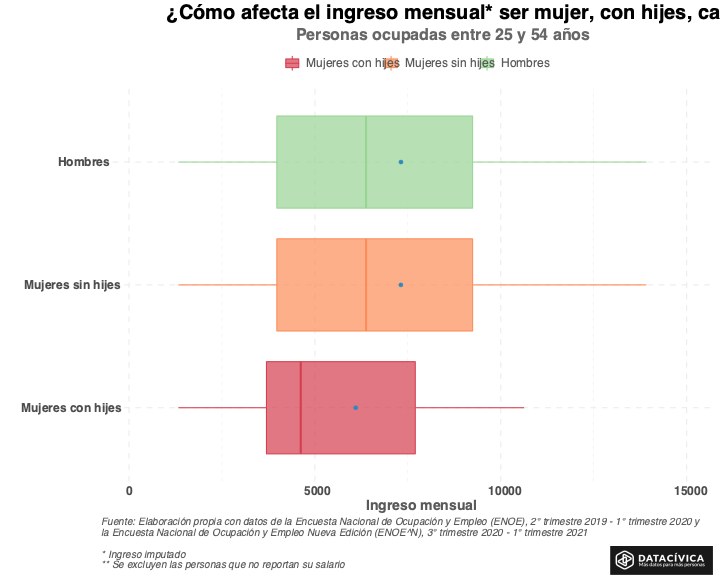
\includegraphics[width=41.67in]{img/boxplot}
\end{frame}

\begin{frame}{¿Cómo los transformamos en cambio?}
\protect\hypertarget{cuxf3mo-los-transformamos-en-cambio}{}
Necesitamos \textbf{interpelar} al usuario:

\begin{itemize}
\tightlist
\item
  Acercándole la problemática

  \begin{itemize}
  \tightlist
  \item
    Personalizando el problema
  \item
    ``TU''
  \end{itemize}
\item
  Reconceptualizando la problemática para dimensionar su magnitud
\item
  Resquematizando los agentes de cambio de la problemática
\item
  Proviendo herramientas para convertir la indignación en acción
\end{itemize}
\end{frame}

\begin{frame}{¿Por qué \textbf{Shiny}?}
\protect\hypertarget{por-quuxe9-shiny}{}
\begin{itemize}
\tightlist
\item
  Recursos limitados de parte del equipo de programación
\item
  Somos científicos sociales que utilizamos R de manera autodidácta
\end{itemize}
\end{frame}

\begin{frame}{OBJETIVO: ¿Cómo utilizar Shiny para generar herramientas
que permitan no solo \textbf{sensibilizar} sino \textbf{tomar acción}?}
\protect\hypertarget{objetivo-cuxf3mo-utilizar-shiny-para-generar-herramientas-que-permitan-no-solo-sensibilizar-sino-tomar-acciuxf3n}{}
\end{frame}

\begin{frame}{¿Cómo \textbf{sensibilizar}? Narrativa: ``Tu huella''}
\protect\hypertarget{cuxf3mo-sensibilizar-narrativa-tu-huella}{}
\begin{columns}[T]
\begin{column}{0.48\textwidth}

\includegraphics{img/group-3.svg}
\end{column}

\begin{column}{0.48\textwidth}
\includegraphics{img/manita_marcador.svg}
\end{column}
\end{columns}
\end{frame}

\begin{frame}{¿Cómo \textbf{sensibilizar}? Narrativa: Niveles del
problema}
\protect\hypertarget{cuxf3mo-sensibilizar-narrativa-niveles-del-problema}{}
\includegraphics[width=1\linewidth]{ppt-LatinR_files/figure-beamer/unnamed-chunk-3-1}
\end{frame}

\begin{frame}[fragile]{¿Cómo \textbf{sensibilizar}? Personalización del
problema}
\protect\hypertarget{cuxf3mo-sensibilizar-personalizaciuxf3n-del-problema}{}
\begin{columns}[T]
\begin{column}{0.48\textwidth}
\href{https://huelladecuidados.datacivica.org/\#Ps-1}{\includegraphics{img/preguntas/p1.png}}
\end{column}

\begin{column}{0.48\textwidth}
\begin{Shaded}
\begin{Highlighting}[]
\NormalTok{mod\_nombreSelect\_ui }\OtherTok{\textless{}{-}} \ControlFlowTok{function}\NormalTok{(id)\{}
\NormalTok{  ns }\OtherTok{\textless{}{-}} \FunctionTok{NS}\NormalTok{(id)}
  \FunctionTok{textInput}\NormalTok{(}\FunctionTok{ns}\NormalTok{(}\StringTok{"nom"}\NormalTok{), }\StringTok{"¿Cuál es tu nombre?"}\NormalTok{, }\StringTok{""}\NormalTok{)}

\NormalTok{\}}
\end{Highlighting}
\end{Shaded}
\end{column}
\end{columns}
\end{frame}

\begin{frame}{¿Cómo \textbf{sensibilizar}? Posicionamiento del usuario
con respecto al resto}
\protect\hypertarget{cuxf3mo-sensibilizar-posicionamiento-del-usuario-con-respecto-al-resto}{}
\href{https://huelladecuidados.datacivica.org/\#mi-huella-1}{\includegraphics{img/preguntas/distri.png}}
\end{frame}

\begin{frame}{¿Cómo \textbf{sensibilizar}? Dimensionando la problemática
de distintas formas}
\protect\hypertarget{cuxf3mo-sensibilizar-dimensionando-la-problemuxe1tica-de-distintas-formas}{}
\href{https://huelladecuidados.datacivica.org/\#mi-huella-3}{\includegraphics{img/preguntas/costop.png}}
\end{frame}

\begin{frame}{¿Cómo \textbf{sensibilizar}? Rendición de cuentas a nivel
local}
\protect\hypertarget{cuxf3mo-sensibilizar-rendiciuxf3n-de-cuentas-a-nivel-local}{}
\href{https://huelladecuidados.datacivica.org/\#municipal-2}{\includegraphics{img/preguntas/scat.png}}
\end{frame}

\begin{frame}{¿Cómo habilitar la \textbf{toma de acción}?}
\protect\hypertarget{cuxf3mo-habilitar-la-toma-de-acciuxf3n}{}
\href{https://huelladecuidados.datacivica.org/\#haz-parte}{\includegraphics{img/preguntas/call2act.png}}
\end{frame}

\begin{frame}{R Markdown}
\protect\hypertarget{r-markdown}{}
This is an R Markdown presentation. Markdown is a simple formatting
syntax for authoring HTML, PDF, and MS Word documents. For more details
on using R Markdown see \url{http://rmarkdown.rstudio.com}.

When you click the \textbf{Knit} button a document will be generated
that includes both content as well as the output of any embedded R code
chunks within the document.
\end{frame}

\begin{frame}{Slide with Bullets}
\protect\hypertarget{slide-with-bullets}{}
\begin{itemize}
\tightlist
\item
  Bullet 1
\item
  Bullet 2
\item
  Bullet 3
\end{itemize}
\end{frame}

\begin{frame}{Slide with R Output}
\protect\hypertarget{slide-with-r-output}{}
\end{frame}

\begin{frame}{Slide with Plot}
\protect\hypertarget{slide-with-plot}{}
\includegraphics{ppt-LatinR_files/figure-beamer/pressure-1.pdf}
\end{frame}

\end{document}
